% !TeX root = report.tex
% !TeX encoding = UTF-8
% !TeX spellcheck = en_US
% !TeX document-id = {b18791db-4bf7-45f4-b2cb-865b91539759}
%
% Report for Street View House Number Recognition
% Udacity MLND Project 5
%
% Aravind Battaje

\documentclass{article}

% Packages used
\usepackage[margin=1in]{geometry}
\usepackage{amsmath}
\usepackage{amsfonts}
\usepackage{multirow}
\usepackage{booktabs}
\usepackage{tabulary}
\usepackage{graphicx}
\usepackage{caption}
\usepackage{subcaption}
\usepackage{url}
\usepackage{hyperref}

% Begin document
\begin{document}
	
	\title{Project Report: Street View House Number Recognition}
	\author{Aravind Battaje}
	\maketitle
	
	\section{Project Overview}
	The project aims to recognize house numbers from images of front of houses taken at street view. One use case this solution could perhaps help is for shipping services that would need to verify delivery by taking a photo at the delivery address and consequently prevent against wrong delivery \cite{news-wrong-address-delivery}; automatic transcription of these pictures could additionally help maintain the records. A (deep) neural network is built to implement a solution for this as a combination of two separately developed models; one to look out for portions of image that contain house numbers, and the other that transcribes the house numbers in these portions. A publicly available dataset \cite{svhn-dataset} is used to train both models, and are finally combined and evaluated against test data. It is found that parts of the solution work very well and with more training, the complete solution can be improved to be used in production settings.
	
	\section{Problem Statement}\label{problem-statement}
	The task in the project is to solve the problem of detecting house numbers, varying from 1 to 5 digits in length, from street view images. This entails recognizing digits in a number of different font styles, sizes, scales and perspective views. Additionally, there might be occlusions or objects in natural scenes that could appear very similar to features in digits, but really might be edges of several shapes that adorn the front view of houses/properties. The solution to this problem can be broken down into two parts: The first part of the solution endeavors to localize or find the region in an image that possibly has digits/house numbers to be recognized (viz., localization). The second part then would work on the localized part of the image to detect the digits reliably (viz., detection). It would make sense to split the solution into the aforementioned two parts rather than having one unified solution as the task of localizing the digits and recognizing the digits could ideally be separated out into two different problems in and of themselves, and more importantly each part could be evaluated and improved independently. Consequently, the localization could perhaps be trained on more (or less) training datasets as compared to the detection part, if the need arises.
	
	Since the detection of multiple digits is a more challenging scenario than the localization, a good strategy would be to first develop a good model to solve the former and possibly use some of the learnings on the latter. Also, the latter could use well known, rather simplistic techniques (\cite{Vaillant94anoriginal}, \cite{SermanetEZMFL13}). In addition to the dataset used in the project to arrive at the final model, a synthetic dataset could also be utilized to simulate some situations that are not prevalent in the real dataset.
	
	Finally, the expected end-solution of the project should be able to reliably detect multiple digits of a house number from street view images that are appropriately sized; the images need not have the digits themselves covering the majority of the area in the picture nor should be having digits covering less than 5\% of the area of the scene.
	
	\section{Metrics}
	As discussed before, since the solution comprises of two rather independent parts, it would make sense to have two different kinds of metrics, especially considering that the localization is a regression kind of problem and detection is a classification task. So, broadly speaking, to evaluate the model of localization, the L2 loss of the predicted region in comparison to the actual region could be used. And for detection, the performance could be evaluated by estimating no-partial-credit accuracy. However, the combined (final) model differs in that the L2 loss is not separately evaluated, but the accuracy and the confidence in the prediction serves as the single metric to evaluate the unified model performance.
	
	In detail, the final model evaluates the no-partial-credit accuracy by considering a prediction as correct only if the length of the predicted digit sequence and each of the digits, in order, matches that of the label. The model also associates a confidence with the prediction, as a relative probability of the predicted outcome -- length and digits -- compared to other combinations of lengths and digits able to be predicted by the model. So, in an extreme case, a low confidence would mean that with slight changes in features in the image, the model could likely predict a different combination of length and digits, in contrast with the current prediction. The confidence, thus, serves as a metric to eliminate predictions that could (probably) be erroneous. The error could be as a result of the detection truly predicting wrongly, or that the localization cutting away parts of the true region, or expanding too much on it.
	
	In the project, the performance of the relatively complex detection is evaluated in the aforementioned form of no-partial-credit accuracy in combination with the confidence; the results with a confidence on predictions below a certain threshold are simply discarded. The performance of the combined model (localization and detection) is also evaluated in a similar manner.
	
	Note that the metrics are evaluated separately for detection model and the combined model because the localization part of the solution suffers from some deficiencies in the dataset (as explained later), and so, evaluating performance of the combined model alone is not very prudent, given the circumstances.
	
	\section{Datasets}\label{datasets}
	The project makes use of two datasets, viz., MNIST \cite{mnist-dataset}\cite{lecun1998}, and SVHN \cite{svhn-dataset}\cite{netzer2011}. MNIST dataset contains a huge number of single digit handwritten characters, in a rather controlled environment -- grayscale, plain background, very low noise etc. SVHN dataset on the other hand is derived from Google Street View images, and contains colored snaps of varying length house numbers in different font styles, lighting conditions, views, textures etc. Although the final model was based mainly on SVHN dataset, the MNIST dataset was used initially to create a synthetic dataset, that simulates multiple digits in a more controlled manner than the SVHN dataset, where the evaluation of model in extreme cases (such as longest length or zero length sequence) couldn't be reliably performed. Table \ref{tab:dataset-length-dist} gives some insight into the imbalance of length of digit sequences in SVHN for the purposes of detection.
	
	The MNIST dataset is provided in two sets, viz., train set and test set. The SVHN dataset is provided in three sets, viz., train set, extra set and test set\footnote{As is the case with most of real-world datasets, there were a few errors found in the dataset labels. This was discovered quite accidentally on few images in the test data set.}. The SVHN dataset, for the purposes of detection was combined into two sets viz., train and extra as (combined) train set, and test set was used as is. The extra set was not used for localization because extra set contains rather simple scenarios with the area of multiple digits data covering the majority of the given image, not really necessitating the function of localization. Additionally, the extra set contains more low-resolution images than train set. For all the datasets and models, a validation set used during the training for hyperparameter tuning was derived as a small percentage (5\% to 10\%) of the (combined) train set. Table \ref{tab:dataset-splits} outlines the number of samples available in each split of the data in different models.
	

	\begin{table}[h]
		\centering
		\begin{tabulary}{\linewidth}{l|CCC}
			\toprule
			& Size of train set (combined, if applicable) & Percentage of train set as validation set & Size of test set \\
			\midrule
			MNIST multi-digit (synthetic) & 69632                                       & 6.25                                      & 16384            \\
			SVHN for detection            & 235755                                      & 5                                         & 13068            \\
			SVHN for localization         & 33402                                       & 10                                       & 13068      		 \\
			\bottomrule      
		\end{tabulary}	
		\caption{Dataset splits}	
		\label{tab:dataset-splits}
	\end{table}
	
	\begin{table}[h]
		\centering
		\begin{tabulary}{\linewidth}{l|CCCCCCC}
			\toprule
			Length                              & 0    & 1    & 2    & 3    & 4    & 5     & 6      \\
			\midrule
			MNIST multi-digit train (synthetic) & 15.7 & 20.7 & 26.5 & 21.1 & 11.1 & 4.9   & NA     \\
			MNIST multi-digit test (synthetic)  & 15.5 & 20.6 & 26.5 & 21.1 & 11.4 & 4.8   & NA     \\
			SVHN train (combined)               & 0    & 6.15 & 38.1 & 48.9 & 6.7  & 0.053 & 0.0004 \\
			SVHN test                           & 0    & 19   & 63.9 & 15.9 & 1.1  & 0.01  & 0                                    \\
			\bottomrule      
		\end{tabulary}	
		\caption{Dataset digit sequence length distribution in percentage}
		\label{tab:dataset-length-dist}
	\end{table}
		
	The MNIST multi-digit datasets are synthetically produced in that varied length of single digits from the MNIST dataset are combined into one image, to produce new combinations of multi-digit sequences. The combining of digits is preceded by random height and width distortions per digit, and random placement of the whole sequence in the combined image. That is, random samples of single digits from MNIST dataset are first distorted randomly on height and width, and then placed side-by-side into a sequence. This sequence is then randomly placed in a 64x64 image, given to the constraint that the combined sequence doesn't get inadvertently cropped. The random distortions were performed to simulate digits with varying scales and font styles, and the random placements were introduced to simulate presence in all parts of the image. The seed used in a Mersenne twister controlling the aforementioned randomization processes is reset at the end of the specified ``dataset size''. Figure \ref{fig:mnist_multi_sample} shows a few samples from the MNIST multi-digit (synthetic) dataset.
	
	\begin{figure}[h]
		\centering
		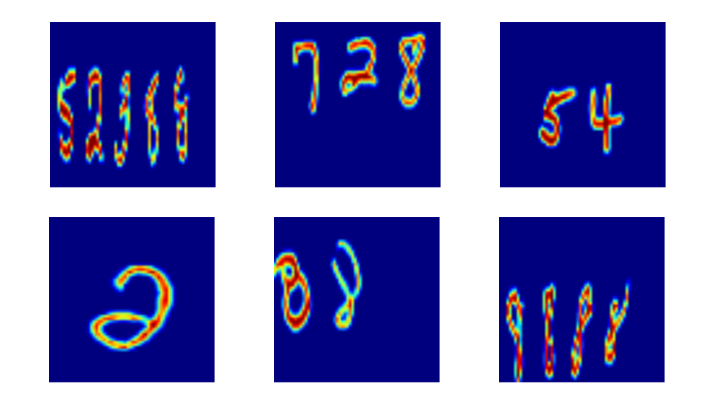
\includegraphics[scale=0.5]{mnist_multi_sample}
		\caption{Samples from MNIST multi-digit (synthetic) dataset}
		\label{fig:mnist_multi_sample}
	\end{figure}
	
	The SVHN dataset used for detection was obtained by primarily cropping the images to the smallest region that contained all digits in the image and scaling that to a fixed size box. In other words, the largest bounding box or the smallest rectangle enclosing all the digits were found from the labels provided with the dataset. This large bounding box was expanded by 30\% on height and 30\% on width, before cropping to it and resizing to a 64x64 image. Data augmentation of placing the digits in slightly different regions of this final image could have been done, but it was found that the variance in labeled bounding boxes and perspective views in the image contributed to producing exact regions of interest in varied positions inherently for SVHN dataset. Figure \ref{fig:svhn_detection_sample} shows a few preprocessed samples from SVHN dataset used for detection.
	
	\begin{figure}[h]
		\centering
		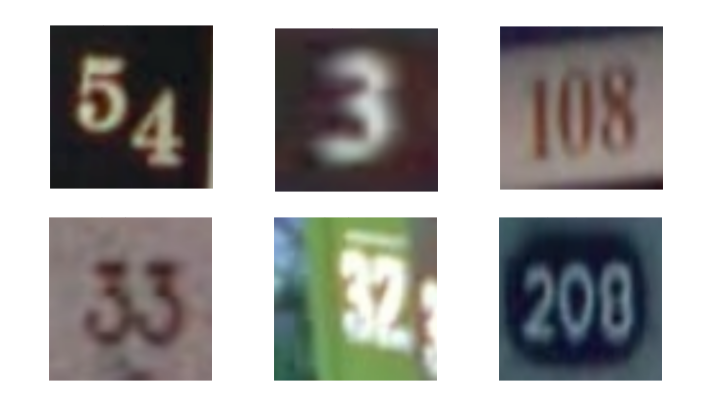
\includegraphics[scale=0.5]{svhn_detection_sample}
		\caption{Sample of SVHN dataset preprocessed to be used for detection}
		\label{fig:svhn_detection_sample}
	\end{figure}
	
	For localization, SVHN dataset was pre-processed in a manner similar to that for detection, but varying in that the large bounding boxes were not expanded and more importantly, the image was never cropped. The images were however resized to a fixed resolution of 80x160, to simulate aspect ratio of 2:1. Unlike the box aspect ratio used for previous types of dataset, 2:1 aspect ratio simulates (or gets close to) typical imaging devices such as smartphone cameras or consumer digital cameras, which would make the localization model easily compatible with images obtained from these sources. It was also found that a box aspect ratio would squish the details too much, if the area containing the digits in an image of the SVHN dataset is less than approx. 25\% of the entire image. Figure \ref{fig:svhn_region_sample} shows a few preprocessed samples from the SVHN dataset used for localization, with the largest bounding boxes overlayed.
	
	\begin{figure}[h]
		\centering
		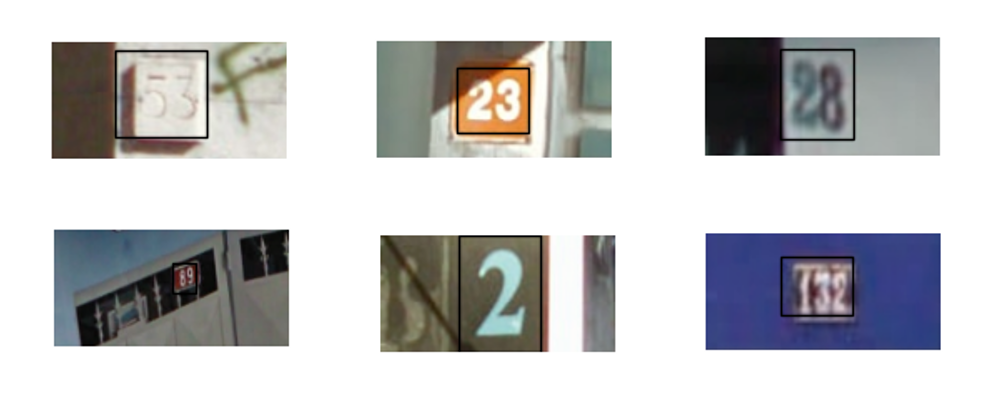
\includegraphics[scale=0.4]{svhn_region_sample}
		\caption{Sample of SVHN dataset preprocessed to be used for localization}
		\label{fig:svhn_region_sample}
	\end{figure}
	
	Common preprocessing applied to all forms of datasets was naive normalization with mean subtraction -- each channel was normalized to 255, and subtracted with 0.5. This doesn't strictly maintain zero mean, but normalizes the range of intensities in each channel to -0.5 to 0.5.	It was found in a preliminary study that more complicated forms of normalization did not provide significant improvements. Finally, the various forms of datasets were encapsulated in classes (called loaders) that primarily produced batches of data to be directly used in the training/evaluation process, in a parallelized manner to promote efficiency.
	
	\section{Detection}\label{detection}
	Given an appropriately cropped (already localized) image, the detection model aims to find the best combination of length and sequence of digits that is present in the input. The basic model for detection is largely based on \cite{GoodfellowBIAS13}, where multiple digit recognition is used to transcribe addresses for use in Google Maps. In \cite{GoodfellowBIAS13}, a maximum accuracy of 96.03\% is achieved on the SVHN test dataset, without considering confidence. The approach taken in this project endeavors to achieve accuracies close to this on SVHN test dataset.
	
	\subsection{Basic model}\label{basic_model}
	The model consists of several convolutional layers processing the raw image inputs into meaningful features, which further gets processed by few fully connected layers. This in turn, is presented as an intermediate form of representation to be used by several classifier ``heads''. The classifier ``heads'' can be divided into two types based on the type of prediction -- length prediction ``head'' and digit prediction ``head''. The model then, as shown in Figure \ref{fig:detection_model}, simply attaches one length prediction head and several digit prediction heads, one for each digit supported, to the last fully connected layer mentioned before. 
	
	\begin{figure}[h]
		\centering
		\includegraphics[scale=0.5]{detection_model}
		\caption{General model for detection}
		\label{fig:detection_model}
	\end{figure}
	
	The prediction done by each classification heads are combined to represent a probabilistic model, as proposed in \cite{GoodfellowBIAS13}. Consider $\mathbf{S}$ as the combined prediction or output sequence, consisting of $L$ as a random variable representing the length of the sequence and $N$ random variables $S_1, ..., S_N$ representing each digit in order. If $X$ is an input image, then, $P(\mathbf{S}|X)$ gives the probability of the output sequence, given the input image, and consequently, the model will be trained to maximize $\log P(\mathbf{S}|X)$ on the training set. The output sequence, given an image, can be further expanded into a joint probability for a prediction of length $n$ and sequence $\mathbf{s} = s_1, ..., s_n$ as
	\[P(\mathbf{S}=\mathbf{s}|X) = P(L=n|X)\prod_{i=1}^{n}P(S_i=s_i|X)\]
	This can also account for inputs having length greater than $N$ by simply enumerating an additional value for $L$ that corresponds to $>N$. Additionally for convenience, we could substitute $H$ in place of $X$ in the above expression, where $H$ is the output of the last fully connected layer. That is, $P(\mathbf{S}|X) = P(\mathbf{S}|H)$, since $H$ must be deterministic for any given $X$ in a feed-forward neural network.
	
	Since the probability variables are discrete, it is feasible to model them as softmax classifiers. All the softmax classifiers (heads) are combined to compute a single loss function, making training similar to one with a single softmax classifier; however, an important distinction is that back-propagation is not carried out on digit classifiers for those inputs that don't have some digits in its label (for length less than $N$). Considering that the labels (one for length, and one for each digit present) are 1-hot encoded, the loss for each softmax classifier can be computed as a cross-entropy product. Thus the training objective of maximizing $\log P(\mathbf{S}|H)$, can be re-interpreted as minimization of loss $ \mathbb{L} = -\log P(\mathbf{S}|H)$. Thus the loss function for a given sequence $\mathbf{s} = s_1, ..., s_n$ of any length $L = n$ for $n <= N$ and $L = N+1$ for $n > N$ becomes
	\[\mathbb{L} = -\log P(L|H) + \sum_{i=1}^{N} -M(S_i = s_i)\log P(S_i = s_i|H) \]
	where $M(\mathbf{S})$ represents ``mask'' for each digit in the sequence, and will simply be 1 for a digit that exists in the sequence and 0 for a digit that doesn't. The masking effectively makes sure that back-propagation only happens on digits that exist in the sequence (label). With this model, the mask is dispensed at test time or simply all assigned to 1. The predicted sequence thus becomes
	\[\mathbf{s} = (n, s_1, ..., s_n) = \arg \max_{L, S_1, ..., S_N} \log P(\mathbf{S}|X) \]
	The confidence in predicting sequence $\mathbf{s}$ is given by
	\[C =  \frac{\max_{L, S_1, ..., S_N} \log P(\mathbf{S}|X)}{\sum_{j=0}^{N+1}\log P(L=j|X) \sum_{i=1}^{N} \max \log P(S_i = s_i | X)}\]
	
	\subsection{MNIST multi-digit detection}
	As already noted in Table \ref{tab:dataset-length-dist}, SVHN dataset has a severe imbalance in the number of examples with different length sequences. the majority of train (combined) dataset is filled by 2 and 3 length digit sequences and there are hardly any examples as it approaches the extremes (0 and 6). To test the validity of the derived model (\ref{basic_model}) at all circumstances, SVHN thus is insufficient. The synthetically created multi-digit dataset on the other hand is much more controllable. As it is apparent in Table \ref{tab:dataset-length-dist}, the MNIST synthetic dataset has a normal distribution with the mean around 2 digits, tailing off quite gracefully toward the extremes of 0 length and 5 length. Note that the model for MNIST multi-digit detection was developed with $L$ taking values $[0,5]$, where 5 is representative of digit lengths greater than 4. Thus the goal of using MNIST multi-digit synthetic dataset was to test the validity of the derived model, and so the emphasis was lesser towards trying to recognize digits in challenging scenarios such as in different lighting conditions, colors etc.
	
	As a precursor to assess the quality of MNIST dataset, a very basic classifier with 2 convolutional layers\footnote{The filter size was fixed at 5x5 with a stride of 1 for all models in this project.} and 1 fully connected layer was modeled on the vanilla (single digit) dataset. All hidden layers had ReLU activation units. The accuracy on this was found to be 99.1\%. The same network was then extended by doubling the number of convolutional and fully connected layers. This feature extraction network was then succeeded by 1 softmax classifier head for predicting length, and 4 softmax classier heads for each digit that was supported. Adam optimizer was used to train the classifier with the loss as derived in \ref{basic_model}.
	
	\begin{figure}[h]
		\centering
		\begin{subfigure}[h]{0.4\textwidth}
			\centering
			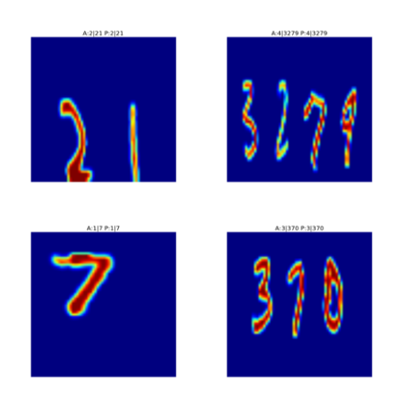
\includegraphics[scale=0.4]{mnist_multi_predict_pos}
			\caption{Correct predictions}
			\label{fig:mnist_multi_predict_pos}
		\end{subfigure}
		\begin{subfigure}[h]{0.4\textwidth}
			\centering
			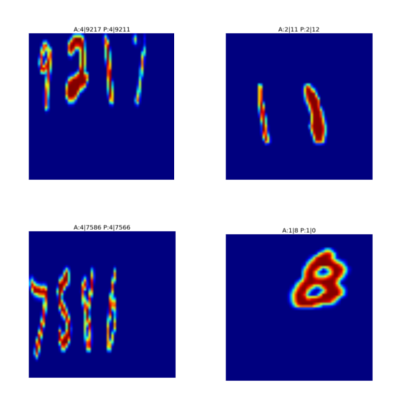
\includegraphics[scale=0.4]{mnist_multi_predict_neg}
			\caption{Incorrect predictions}
			\label{fig:mnist_multi_predict_neg}
		\end{subfigure}
		\caption{MNIST multi-digit model predictions on synthetic dataset. In \ref{fig:mnist_multi_predict_neg}, clockwise from top-left: A:4|9217 P:4|9211; A:2|11 P:2|12; A:4|7586 P:4|7566; A:1|8 P:1|0, where A is actual label, P is predicted label, and the character ``|'' separates length and digits sequence respectively.}
	\end{figure}
	
	After some (not so rigorous) hyperparameter tuning, the final model for MNIST multi-digit detection achieved 97\% accuracy on the test dataset, after about an hour\footnote{All the training for this project was carried out in AWS g2.2xlarge instance with NVIDIA GRID K520 GPU.} of training. Confidences were not extracted or used to evaluate performance at this point as confidence is only a ratio of relative probabilities, and wouldn't directly help assess effectiveness of the derived model. The accuracy of 97\% is impressive, considering that the synthetic dataset produced certain distortions that were hard to even manually decipher. Figure \ref{fig:mnist_multi_predict_pos} and \ref{fig:mnist_multi_predict_neg} show few correctly and incorrectly predicted examples from the test (synthetic) dataset respectively. More evaluation results for this model can be found in the project repository \cite{mnist-multi-eval}. Ostensibly, in the incorrect predictions, the model gets almost all details correct except one or two digits in the sequence, which when individually taken produce incorrect predictions with the single digit (precursor) classifier too, and there are hardly any examples with wrong length prediction. Importantly, the model also predicts the extremities -- 0 length and $ >4 $ length sequences -- reliably.
	
	Thus the derived probabilistic model (\ref{basic_model}) to predict multiple digits seems to be a very good fit for recognizing multiple digits in house numbers. 
	
	\subsection{SVHN detection}\label{svhn_detection}
	The model used for MNIST multi-digit detection was extended to make a total of 6 convolutional layers and 3 fully connected layers, terminating with the length and 5 digits softmax classifiers. Note that this model extended the number of supported digits by one, and so, $L$ had 7 different outputs $[0,6]$ with 6 corresponding to sequence length greater than 5 digits. Unlike in the MNIST models where max pooling\footnote{Max pooling was fixed at 2x2 filter with a stride of 2 for all models in the project.} was applied after every convolutional layer, they were now interspersed alternatively for the first 4 convolutional layers, followed by max pooling for both fifth and sixth convolutional layers. The model needed to become deeper because in contrast with MNIST multi-digit, the input transformations had to be done in more elaborate conditions before being processed by individual softmax classifiers, such as with noise and different lightings that would require more processing for example on edge gradients (convolutional layers); various orientations and arrangements that would require more complex affine transformations (fully connected layers) etc.
	
	\begin{figure}[h]
		\centering
		\begin{subfigure}[h]{0.4\textwidth}
			\centering
			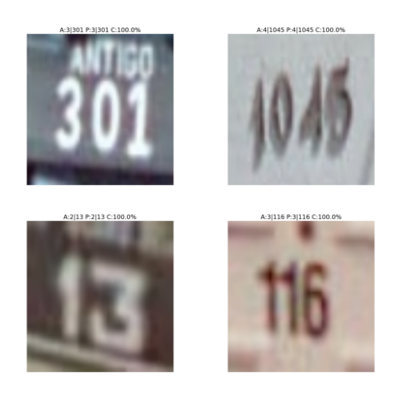
\includegraphics[scale=0.4]{svhn_multi_predict_pos}
			\caption{Correct predictions}
			\label{fig:svhn_multi_predict_pos}
		\end{subfigure}
		\begin{subfigure}[h]{0.4\textwidth}
			\centering
			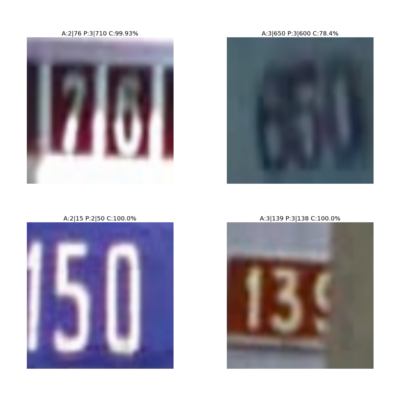
\includegraphics[scale=0.4]{svhn_multi_predict_neg}
			\caption{Incorrect predictions}
			\label{fig:svhn_multi_predict_neg}
		\end{subfigure}
		\caption{SVHN detection model predictions on SVHN test dataset. In \ref{fig:svhn_multi_predict_neg}, clockwise from top-left: A:2|76 P:3|710 C:99.93\%; A:3|650 P:3|600 C:78.40\%; A:3|139 P:3|138 C:100.0\%; A:2|15 P:2|50 C:100.0\%, where A is actual label, P is predicted label, and the character ``|'' separates length and digits sequence respectively; C is confidence in the prediction.}
	\end{figure}
	
	The hyperparameter tuning with validation was done manually by first finding the apt number of filters in each convolutional layer, with a constant learning rate. It was followed by fixing the number of hidden neurons for each layer in the fully connected network. This was followed by different combinations of dropout and its keep probability in the hidden layers. Finally, the apt learning rate was found and the final model was trained on approx. 8 epochs of the SVHN combined train data. By this time, accuracy on test dataset reached 91.57\%. Training was resumed on a higher proportion of SVHN train set (i.e., more number of samples from SVHN train set compared to the SVHN extra set) for 8 epochs with a learning rate 5 times lower than initially used with the combined set. After a combined 5 hours of training, accuracy on test dataset was 91.75\%. This ``augmentation'' was necessary to prevent overfitting on the fully combined dataset that had more than 10 times the number of examples from the extra set then the train set; the former being slightly less ``challenging'' than the latter. During ``augmentation'', the ratio was brought down to 5 samples from train set with 1 sample from extra set. Slightly better accuracy on the test dataset of 94\% can be obtained by rejecting samples lesser than 98\% confidence.
	
	Figure \ref{fig:svhn_multi_predict_pos} shows some correct predictions on the test dataset, and it can be seen that the model has learnt to pick out numbers in challenging scenarios, such as the top-left prediction which has ``noise'' from characters on top of the digits. From the other samples, it can also be seen that the prediction is robust against multiple colors, views, shadows etc. The confidence attached to each of these predictions shown were 100\% too. Figure \ref{fig:svhn_multi_predict_neg} shows a few incorrect predictions. Several pitfalls and caveats to the model/dataset become apparent here: The top-left sample has been predicted with 99.93\% certainty to be the digit sequence 710 instead of the actual 76. One could argue that cropping of images to this zoom level could even confuse a human reader, because enough context about each digit embedded in separate red squares is not present, which makes the middle separator between the red squares appear like a digit 1. The top-right sample is not very clear in that it lacks good resolution; the model thus predicts this to be 600 instead of the actual 650 with only 78.4\% certainty. The bottom-right sample is a good case of partial occlusion, in that the model has to ``figure out'' the rest of the third digit in the picture. More samples or a deeper network could help address this problem. The bottom-left sample could clearly be a case of mis-labeling, where one could argue that actual digit sequence is 150, but has been labeled as 15. Additionally since the first digit is at the borders, and might very well be part of some texture instead of the digit itself, the model has ignored this digit and predicted the last two digits as 50 with 100\% certainty Apart from the apparent mis-labeling, these kind of situations could potentially be solved with better localization (and thus cropping). More evaluation results for detection model can be found in the project repository \cite{svhn-multi-eval}.
	
	\section{Localization}\label{localization}
	The recognition of digit sequences in input images that are already cropped to approximate region of the digits in a full image has already been discussed in \ref{detection}. Practically however, a holistic approach of recognizing digit sequences in an arbitrary image would be a more complete solution. So a method for localization of possible candidates that the SVHN detection model (\ref{svhn_detection}) could work on, was developed. Ideally, a localization algorithm could produce multiple candidates if there are multiple regions of interest in an arbitrary image, or produce multiple candidates (slightly shifted) for a single region of interest for obtaining better confidence. In the project however, the localization is limited to a single region of interest for a given image, both due to simplicity of the combined model used, and because of dataset limitations. The dataset was limited in that there weren't many examples in SVHN dataset with the house numbers (region of interest) themselves covering a small area in the full image, and with high spatial variation.
	
	\begin{figure}[h]
		\centering
		\includegraphics[scale=0.5]{localization_model}
		\caption{General model for localization}
		\label{fig:localization_model}
	\end{figure}
	
	The convolutional layers trained in \ref{svhn_detection} can be seen as feature extractors specialized to extract features pertaining to digits in different natural scenes. The fully connected layers succeeding the convolutional layers would then transform the extracted features in spatial domain to be consumed by the several classifier heads. Since the localization model should find candidate locations of digits in a bigger image, and localize a bounding box around this region of interest, the convolutional layers already trained in \ref{svhn_detection} could be reused to find the features relevant to digits in an arbitrary image and a separately trained fully connected network could be utilized to transform the features differently (compared to detection) and predict a bounding box. Figure \ref{fig:localization_model} shows the general model for localization using convolutional layers from detection model. It should be noted however that the input/arbitrary images shouldn't have resolutions that are too different to what the detection model learned on. In other words, if the convolutional layers for detection model were trained on images of size 64x64, it wouldn't make sense to reuse this model on images which are say 10 times bigger on each dimension (640x640) as the features themselves could be upscaled beyond recognition. The same holds true for downsized images. So the localization model will be constrained to use image resolutions that are not too different from the one used for detection model, if the convolutional layers are reused. It was found, even with this constraint however, that a resolution of 80x160 was not too restrictive for arbitrary images from the SVHN dataset. The choice of aspect ratio 2:1 has already been explained in \ref{datasets}.
	
	The fully connected network succeeding the pretrained convolutional layers contained 2 hidden layers with dropout, ending with 4 neurons, each corresponding to the top, left, width and height of the bounding box prediction respectively. Since this is a classic regression task, a loss similar to the typical L2 loss, was derived for training the fully connected network. The loss was differing only in that it was a form of weighted L2 loss and it dispensed of the square root for simplicity:
	\[\mathbb{L} = 2(t_l - t_p)^2 + 2(l_l - l_p)^2 + (w_l - w_p)^2 + (h_l - h_p)^2 \]
	where $t_l$, $l_l$, $w_l$, $h_l$ and $t_p$, $l_p$, $w_p$, $h_p$ are label (actual) and predicted top, left, width and height respectively. As in the case of previous models, Adam optimizer was used to train with this loss.
	
	As already mentioned in \ref{datasets}, training was only carried out on SVHN train set (without combining with the extra set) for localization as the extra set didn't have a lot of variation in position and size of region of interest. The training time was heavily cut down because of pretrained convolutional layers -- the final model took only about 30 minutes to train. However, even with rigorous hyperparameter tuning, the network tended to overfit very quickly on training set. This can be attributed both to the reduced size of training corpus, and the absence of a good amount of position variance to suit the task of localization. To counter this, training was first performed with a high learning rate exclusively on train dataset for approx. 4 epochs, and then training on the network was shifted to test dataset for approx. 4 epochs with a low learning rate. This may be considered ``cheating'' in the truest sense, but this was essential to get some decent performance. Ironically, the test dataset contained more challenging scenarios than the train dataset in terms of positional variance, which was apparent when complete training was performed on a switched dataset, i.e., the SVHN test set was considered as the train set, and the SVHN train set was considered as test set. The loss with this setting was almost 2 times lower on the test set (in reality, SVHN train set) than the normal (not switched dataset) setting. The average loss on the test data set with the 2-phased training was around 200 per image. This metric is not really representative of the true performance of the network as part of the training is performed on the test dataset albeit with a very low learning rate. The true performance was only subjectively evaluated with a set of 30 images downloaded separately from Google Maps \cite{google-street-view-samples}, on which the model could be said to have predicted decent bounding boxes for about 70\% of images. Some sample bounding box predictions can be seen in Figure \ref{fig:combined_predict}.
	
	With the above mentioned caveats, the training for localization can be still considered inadequate, and so the model can only be considered representative and not worthy to be used in a real world setting, unless more data is available. The predicament is corroborated by the fact that there were no samples in the SVHN dataset with zero-length digits (refer Table \ref{tab:dataset-length-dist}), which is essential for a localization model to further differentiate if there is any digits (region of interest) at all in an arbitrary image. Only with some dataset that provides many images with street view images sans the house numbers would truly be able to cover this area for the localization model. 
	
	As an aside, an experiment was conducted by retaining the same convolutional layer network from the detection model but without the pre-training. This ``fresh training'' approach didn't perform much better in terms of overfitting or final model performance than the one presented above. This further ascertains the point that SVHN train set alone is not a good candidate for training a network for reliable localization.
	
	\section{Combined model}\label{combined_model}
	To implement an end-to-end solution, the localization model (\ref{localization}) and the detection model (\ref{detection}) were combined into a single network. Input images, were resized to 80x160 and fed to the localization network. The region in the input image as predicted by the localization network was expanded by a specific amount, cropped and resized to 64x64. This resized image was fed to the detection model to predict the digit sequence. Figure \ref{fig:combined_model} illustrates a generalized model combining the localization and detection models. Note that the convolutional layer is only trained once during training of detection model, and then re-used during the training of localization model.
	
	\begin{figure}[h]
		\centering
		\includegraphics[scale=0.4]{combined_model}
		\caption{General model for localization and detection combined}
		\label{fig:combined_model}
	\end{figure}
	
	If all aspects of this combined model were to be evaluated, it would seem quite tricky as detection is directly dependent on localization and performance of the latter would inadvertently affect former. So the evaluation here is performed by looking at the results of digit sequence prediction and its confidence. If a digit sequence is predicted with a sufficient enough confidence, it is then evaluated for accuracy. So the accuracy for the combined model with a 30\% expansion of predicted bounding box by localization, is 69.9\% with 99\% confidence thresholding on the SVHN test dataset. This result is dismal compared to the much better performance of the detection model alone, but with better localization model, the combined accuracy could surely go up. Figure \ref{fig:combined_predict_pos} shows some correctly predicted samples using the combined model. It is apparent from the top-right and bottom-right samples, that the localization is not really as good as it could be (subjectively), and yet the detection model is able to get the digit sequence right, although the top-right sample with confidence of 98.61\% will be discarded by the evaluation metric. On the plus side, the bottom-right and top-left samples serve as moderately challenging scenarios to localize, and images like these can't be expected to be deciphered by detection model alone. Figure \ref{fig:combined_predict_neg} contains few incorrectly predicted examples, and it is apparent in all of them that the prediction suffers mainly because of the bad localization. The top-left and bottom-left images have been localized to too small and too large area, but fortunately, the confidences are low (54.55\% and 96.91\% respectively), which would get discarded in the confidence thresholding. Unfortunately, the top-right and bottom-right samples have been localized at wrong regions, forcing the detection model to predict wrong digit sequences with 100\% certainty. More evaluation results for the combined model can be found in the project repository \cite{combined-eval}.
	
	\begin{figure}[!ht]
		\centering
		\begin{subfigure}{\textwidth}
			\centering
			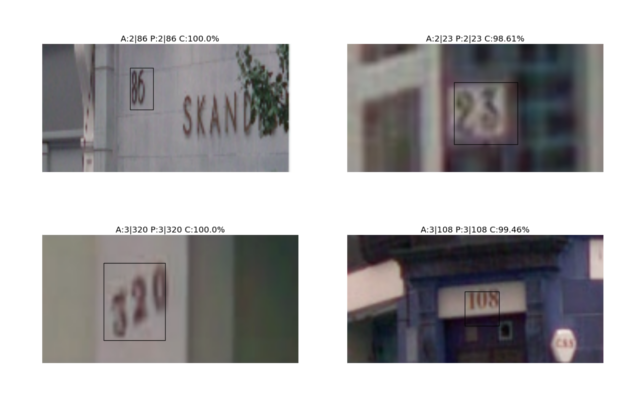
\includegraphics[scale=0.6]{combined_predict_pos}
			\caption{Correct predictions}
			\label{fig:combined_predict_pos}
		\end{subfigure}
		\begin{subfigure}{\textwidth}
			\centering
			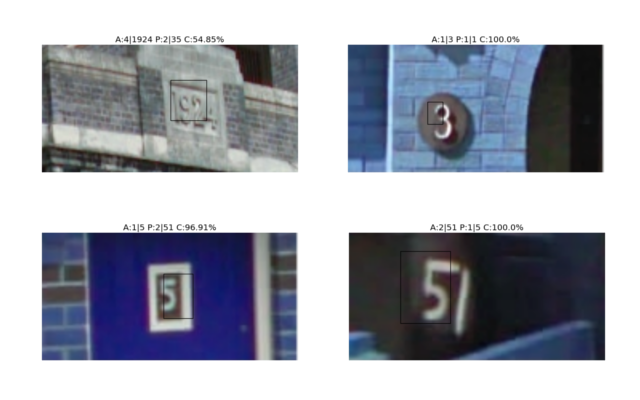
\includegraphics[scale=0.6]{combined_predict_neg}
			\caption{Incorrect predictions}
			\label{fig:combined_predict_neg}
		\end{subfigure}
		\caption{Combined model predictions on SVHN test dataset. In title of each image, A is actual label, P is predicted label, and the character ``|'' separates length and digits sequence respectively; C is confidence in the prediction.}
		\label{fig:combined_predict}
	\end{figure}
	
	Finally, running the model on a low-powered PC (Core i3 CPU) takes on an average 360 ms per image, and about 400 MB of memory in total when fully loaded. This can be regarded as a light-weight model, given that further reduction can be achieved with fixed point numbers and such quantization in TensorFlow.
	
	\subsection{Google Street View images}
	To evaluate performance of the localization model on never-before-seen data, and to demonstrate generalization of the combined model on arbitrary images, some images from Google (Maps) Street View were downloaded \cite{google-street-view-samples}. Some results are shown in Figure \ref{fig:sample_predict}. It is apparent that the sample predictions suffer from the same kind of problems with localization as already mentioned in \ref{combined_model}. Alternatively, the accuracy of the detection model on manually cropped sample images was 93.1\% with a confidence threshold of 99\%, which is close to the accuracy on SVHN test dataset. (However, it is important to note that there are only 30 images in the sample set, and so, the performance is merely representative.) This further corroborates the weakness of the localization model, but on the flip side, the detection model can be said to have achieved sufficient generalization.
	
	\begin{figure}[h]
		\centering
		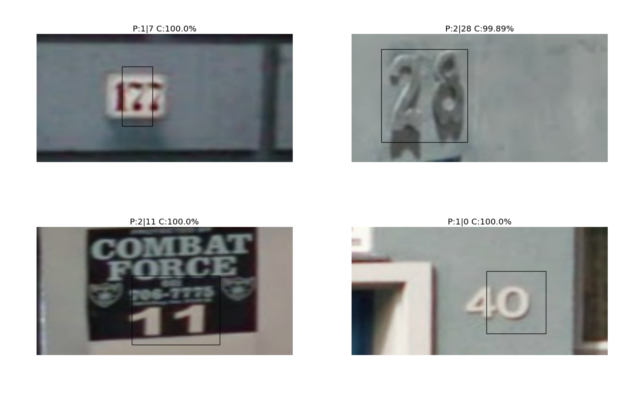
\includegraphics[scale=0.6]{sample_predict}
		\caption{Combined model sample predictions on Google (Maps) Street View images}
		\label{fig:sample_predict}
	\end{figure}
	
	\section{Hyperparameter tuning process}
	Hyperparameter tuning is the process of selecting the apt hyperparameters, such as choice of optimizer, learning rate, number of nodes in a hidden layer, number of convolution filters in a layer etc., for a given broad neural network architecture. This process could easily be said as the hardest and most time-consuming. However, several recent work in this field has made this process simpler; the amount of options left to be tuned was minimized by using some of these work. Adam optimizer \cite{KingmaB14}, a learning rate adaptive, momentum-based stochastic gradient descent method was used for training with models' loss functions. ``Xavier'' \cite{Glorot10}, and ``He'' \cite{HeZR015} weight initializations were tried to improve convergence, and ``He'' was found to be suitable.
	
	Unlike the recommendation of randomly searching \cite{Bergstra2012} for the remaining hyperparameters such as initial learning rate, number of epochs, depth/width of each layer, etc., only a manual search was done, both due to computing (monetary) resource constraints, and to develop intuition for some parameters. TensorBoard utility of the TensorFlow library immensely helped in doing this manual process. Statistics about variables in the network such as their distribution and mean, and zero-fraction of activation functions were logged for each ``run'' of a particular model and monitored live. For example, zero-fraction helped in finding if some process had inadvertently created many ``dead''-neurons, and validation accuracies showed overfitting tendencies, if any. Model checkpoints were also regularly created, in case the model crashed due to some reason or early exit was required, such as in the case of localization model where the variables at some steps before the last training step was considered instead of the last step. Finally, models with higher complexity (or deeper networks) were not tried exhaustively due to the above said resource constraints.
	
	\section{Conclusion and Improvements}
	The intention of the project was to try to achieve an end-to-end solution for recognizing house numbers from arbitrary image inputs, possibly from a smartphone or a digital camera. The project developed a suitable model to achieve this goal, and the model is also aptly cheap enough to be run on smartphones. The detection model's accuracy of 91.75\% sequence transcription accuracy on SVHN test dataset can be said to have achieved a performance close to the model it was based on \cite{GoodfellowBIAS13}, considering the resource constraints. Finally, although the localization model has its weaknesses, with a better dataset to train for localization, higher overall performance could most likely be achieved.
	
	As already mentioned in \ref{problem-statement}, the modularity of models maintained in this project is crucial to improve upon each independently. The detection model could be improved to support more characters typically available in house numbers apart from digits, such as ``/'' (bar) and first few letters of the alphabet. The model complexity could also be increased, as implemented in \cite{GoodfellowBIAS13}, to increase accuracy, albeit at a slightly higher inference computation cost. On the other hand, the localization (and in turn the combined) model could be made more robust for multiple regions of interests (or multiple groups of digits in a single image) by having the localization produce multiple candidates. It could additionally work on different scales of an input image to catch regions of interest that is too big or too small. Implementing these improvements would undoubtedly need much more complex and vast dataset.
	
	\section{Reflections and Acknowledgments}	
	In the project development process, the hyperparameter tuning and building model architectures were particularly very insightful and provided deep understanding of neural networks.
	
	Udacity's Deep Learning course coupled with Stanford's CS231n course \cite{cs231n} were essential in understanding deep neural networks in a working level detail. TensorFlow library along with its utilities and excellent documentation \cite{tensorflow-doc} aided in quickly realizing stable and reusable computational graphs used in the entire project. High performance computing cloud solutions provided by Amazon Web Services was instrumental in quickly prototyping and trying out several model architectures for this project. Finally, the wizards who made Python and NumPy possible deserve the utmost respect for allowing to work on complex projects and take it to completion within weeks.
	
	\bibliographystyle{ieeetr}
	\bibliography{report}
\end{document}